\documentclass{asaproc}

\usepackage{dsfont}
\usepackage{graphicx}
\usepackage{bm}
\newcommand{\m}[1]{\mathbf{\bm{#1}}}
\newcommand{\R}{I\hspace{-4.4pt}R}

%\usepackage{times}
%If you have times installed on your system, please
%uncomment the line above

%For figures and tables to stretch across two columns
%use \begin{figure*} \end{figure*} and
%\begin{table*}\end{table*}
% please place figures & tables as close as possible
% to text references


\newcommand{\be}{\begin{equation}}
\newcommand{\ee}{\end{equation}}

\title{FYE Take Home (Statistics)}

%input all authors' names

\author{ID: 709}

%input affiliations

%{USDA Forest Service Forest Products Laboratory}

\begin{document}

\maketitle

\begin{abstract}
The data set we explore in this paper consists of daily measurements of ozone concentration, solar radiation, maximum temperature, and wind speed. We develop two Bayesian regression models to explain ozone concentration: one based on only temperature and wind speed and the other based on all three covariates. The deviance information criterion (DIC) and other measures are used to analyze the fit of and compare the models. Despite the two models performing very similarly, we prefer the slightly more complicated model which uses radiation as a predictor.
\end{abstract}

\section{Introduction}

The primary focus of this paper is to explore how solar radiation, maximum temperature, and wind speed relate to ozone concentration. The data set we use consists of 111 daily observations for each of these variables. Solar radiation is measured as either 0 (for low) or 1 (for moderate or high levels), temperature is in degrees Fahrenheit, wind speed is in miles per hour, and ozone is in units of parts per billion.

In section 2, we perform an exploratory analysis of the data and offer motivation behind our model choice. In section 3, we discuss our modeling approach and the methods used in selecting and analyzing the models. Results are provided in section 4 and we conclude with a discussion in section 5.

\section{Exploratory Analysis}

A 3-dimensional plot of the data is shown in Figure \ref{data}. In that plot, temperature and wind speed make up the $x$- and $y$-axes while the response (ozone) is on the $z$-axis. The color of the dot marks the radiation, black for low and red for moderate or high. This plot gives us quite a bit of information about how the covariates are related to each other and to the response. There is a pattern that high ozone concentration is associated with high temperature, low wind speed, and moderate or high radiation level. These seem to have a tendency to all occur together, suggesting some degree of interaction.

\begin{figure}
\begin{center}
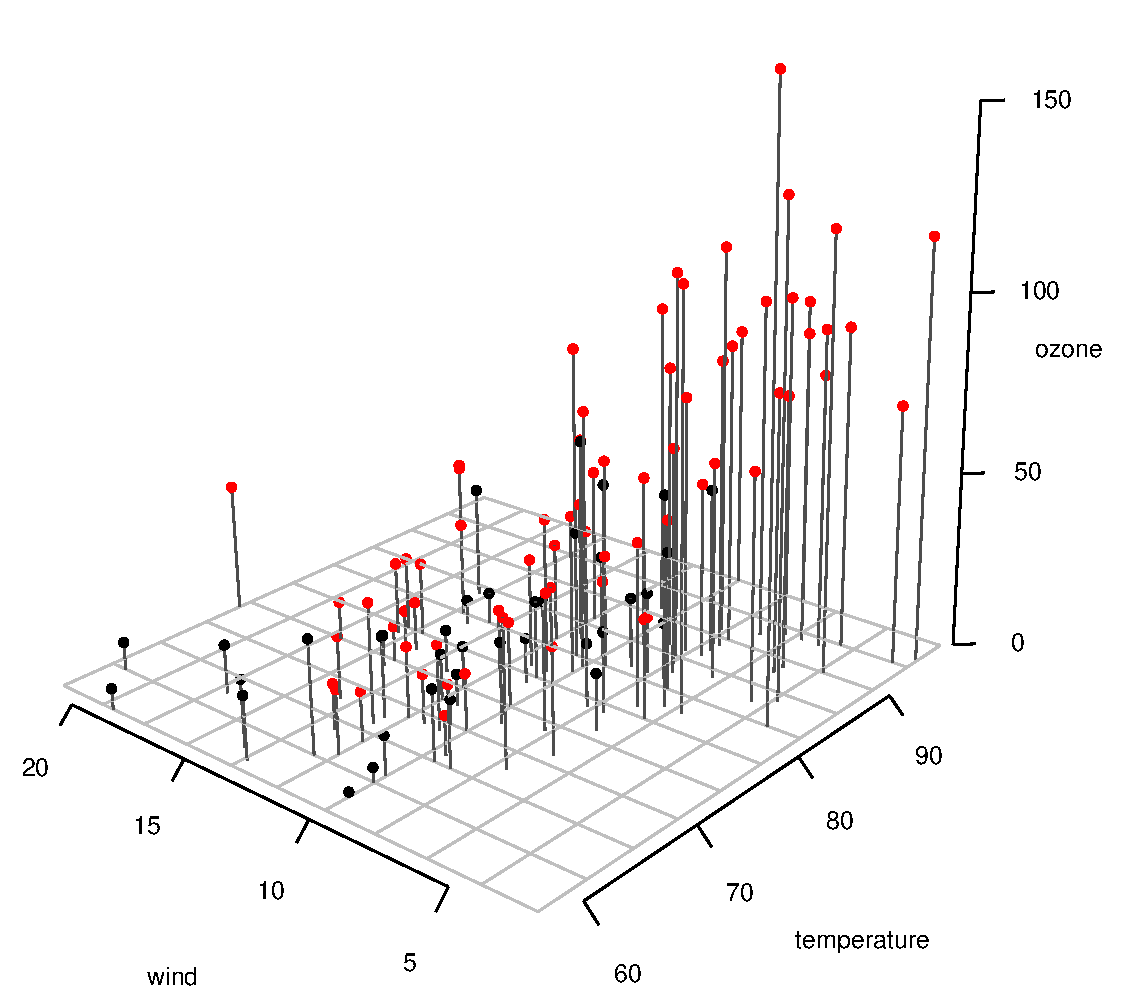
\includegraphics[scale=0.44]{figs/crop_data.pdf}
\caption{3-dimensional plot of the data on its original scale. The red dots indicate observations with moderate or high radiation levels ($R_i=1$) and black are for low radiation ($R_i=0$).}
\label{data}
\end{center}
\end{figure}

\begin{figure}
\begin{center}
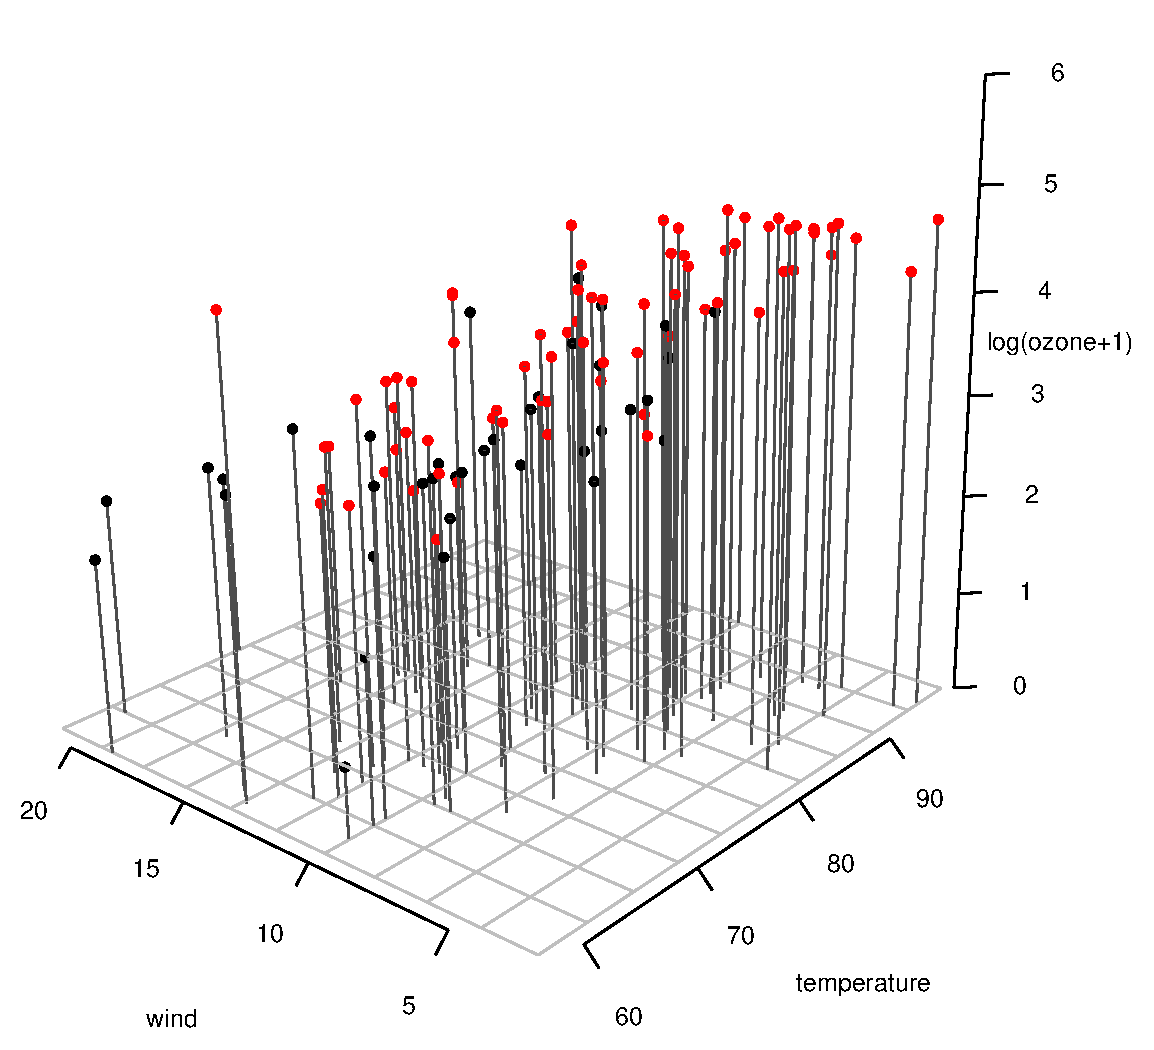
\includegraphics[scale=0.44]{figs/crop_log_data.pdf}
\caption{3-dimensional plot of the data with the transformed response $\log(ozone + 1)$.}
\label{log_data}
\end{center}
\end{figure}

\begin{figure}
\begin{center}
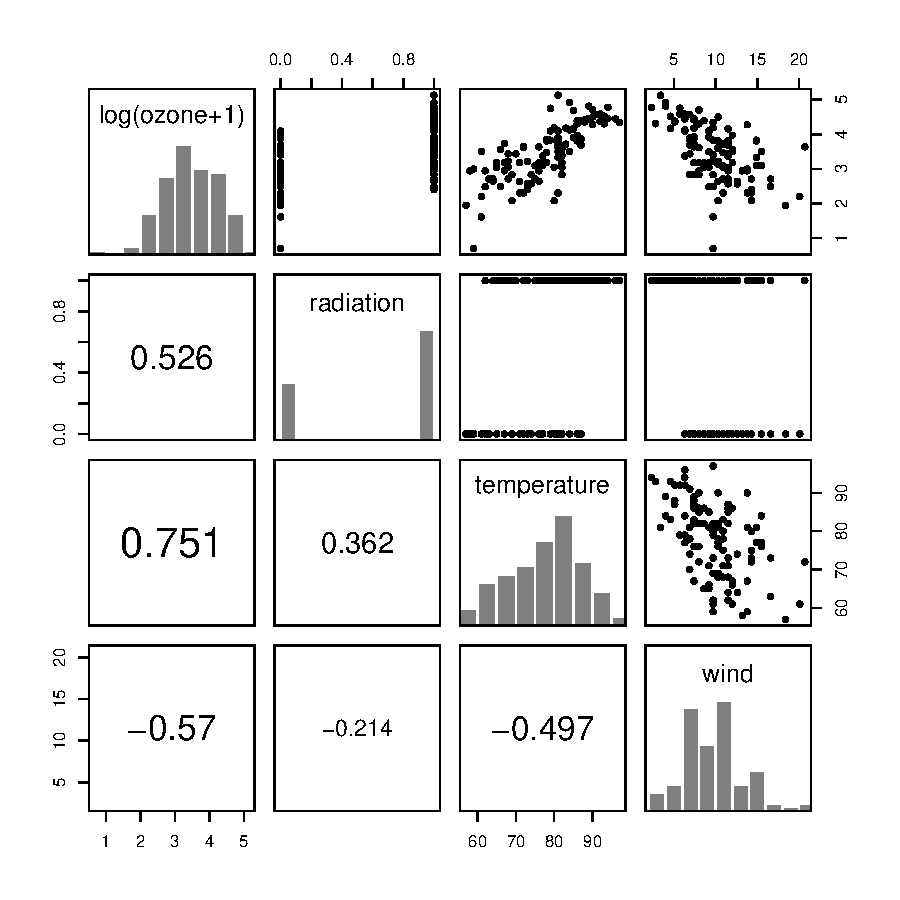
\includegraphics[scale=0.55]{figs/pairs.pdf}
\caption{\emph{Diagonal}: histograms for marginals of each variable. \emph{Upper diagonal}: two-way plots for each combination of variables. \emph{Lower diagonal}: sample correlation.}
\label{pairs}
\end{center}
\end{figure}

Though not shown, plots of temperature against ozone and wind speed against ozone showed non-linear associations and heteroscedasticity. The non-linear relationship between covariate and response can be modeled with linear combinations of basis functions such as splines, but this does not necessarily deal with the non-constant variance problem. To deal with the variance, we take the log transformation of the response (specifically, we let our new response be $y=\log(ozone+1)$, where the $+1$ accounts for cases with $ozone=0$). The transformed data are shown in Figure \ref{log_data}. The transformation does making interpretation of model parameters difficult, but most of the heteroscedasticity issue is now absent.

With the 3-d plot alone, it could be difficult to decide on a regression model. To select how we wish to relate the covariates to the response, we look at the pairs plot (Figure \ref{pairs}). From this set of plots, we see how each covariate is related (marginally) to the response. We confirm the original finding that high temperature, low wind speed, and high radiation are associated with high ozone. The transformation has also made the relationships between covariate and response more linear. This prompts us to consider basic regression models.

\section{Methods}

\subsection{Regression model}

In this paper, we consider several models, each of which has the form
\[ \m{y}|\m{\beta},\sigma^2 \sim N\left(\m{X}\m{\beta}, \sigma^2\m{I}\right) \]
where $\m{y}=(y_1,\ldots,y_n)^\top$, $n=111$, is the vector of transformed ozone levels, $\m{X}$ is the $n\times p$ design matrix, $\m{\beta}$ the $p$-vector of model parameters, $\sigma^2$ the observation error, and $\m{I}$ is the $n\times n$ identity matrix. Priors on $\m{\beta}$ and $\sigma^2$ will be discussed in the next section.

Let $\m{r}$ be the binary vector denoting the category of radiation level (0 for low, 1 for moderate or high), $\m{T}$ be the vector of temperatures in degrees Fahrenheit, and $\m{w}$ the vector of wind speed in miles per hour. Each vector is of length $n$. We will construct a total of 18 models (18 different $\m{X}$ matrices) made up of the various combinations of $\m{r}$, $\m{T}$, and $\m{w}$ and their first-order interactions. The complete list is given in Table \ref{models}. Such a wide array of models enables us to look at the impact of each term. Of course, doing model comparison in this way is only feasible because of the simpleness of the models. This certainly will not work for complicated models or with large data sets.

Though we consider several models, we will narrow it down to two: one without a radiation component (M1) and one with a radiation component (M2). These will be selected based on their deviance information criterion (section 3.4). M1 will be selected from those models which have no radiation component included (there are five such models listed in Table \ref{models}). M2 will be selected from all 18.

\begin{table}
\caption{Design matrices $\m{X}$ for the 18 models. The notation $\m{u}\circ\m{v}$ denotes element-wise multiplication.}
\centering
\begin{tabular}{ll}
\\ [-5pt]
\hline \hline
$\m{X}$                                     & $\m{X}$   \\ \hline
$(\m{1}_n)$                                 & $(\m{1}_n, \m{T}, \m{w}, \m{T}\circ \m{w})$ \\
$(\m{1}_n, \m{r})$                          & $(\m{1}_n, \m{r}, \m{T}, \m{w})$ \\
$(\m{1}_n, \m{T})$                          & $(\m{1}_n, \m{r}, \m{T}, \m{w}, \m{r}\circ \m{T})$ \\
$(\m{1}_n, \m{w})$                          & $(\m{1}_n, \m{r}, \m{T}, \m{w}, \m{r}\circ\m{w})$ \\
$(\m{1}_n, \m{r}, \m{T})$                   & $(\m{1}_n, \m{r}, \m{T}, \m{w}, \m{T}\circ \m{w})$ \\
$(\m{1}_n, \m{r}, \m{T}, \m{r}\circ \m{T})$ & $(\m{1}_n, \m{r}, \m{T}, \m{w}, \m{r}\circ \m{T}, \m{r}\circ\m{w})$ \\
$(\m{1}_n, \m{r}, \m{w})$                   & $(\m{1}_n, \m{r}, \m{T}, \m{w}, \m{r}\circ \m{T}, \m{T}\circ\m{w})$ \\
$(\m{1}_n, \m{r}, \m{w}, \m{r}\circ \m{w})$ & $(\m{1}_n, \m{r}, \m{T}, \m{w}, \m{r}\circ \m{w}, \m{T}\circ\m{w})$ \\
$(\m{1}_n, \m{T}, \m{w})$                   & $(\m{1}_n, \m{r}, \m{T}, \m{w}, \m{r}\circ \m{T}, \m{r}\circ\m{w}, \m{T}\circ\m{w})$ \\ \hline\hline
\end{tabular}
\label{models}
\end{table}

\subsection{Priors for $\m{\beta}$ and $\sigma^2$}

We use a Zellner's $g$-prior for $\m{\beta}$ and $\sigma^2$:
\begin{eqnarray*}
\m{\beta}|\sigma^2 &\sim& N\left(\m{m}, g\sigma^2(\m{X}^\top\m{X})^{-1}\right) \\
p(\sigma^2) &\propto& (\sigma^2)^{-1}
\end{eqnarray*}
This informative prior distribution on $\m{\beta}$ incorporates the design matrix $\m{X}$. Specifying a reasonable prior covariance for $\m{\beta}$ can be difficult, but $(\m{X}^\top\m{X})^{-1}$ provides a decent solution without much effort on our part. We complete the prior by choosing $\m{m}=\m{0}$ and fixing $g=n$.

This specification produces the following posterior full conditionals
\begin{eqnarray*}
\m{\beta}|\sigma^2, \m{y}, \m{X} &\sim& N\left(\frac{1}{g+1}(g\hat{\m{\beta}}-\m{m}), \frac{g\sigma^2}{g+1}(\m{X}^\top\m{X})^{-1}\right) \\
\sigma^2|\m{\beta}, \m{y}, \m{X} &\sim& IG\left(\frac{n}{2}+\frac{p}{2}, \frac{1}{2}(\m{y}-\m{X}\m{\beta})^\top(\m{y}-\m{X}\m{\beta})\right.+ \\
& & ~~~~ ~~~~ ~~~~ \left.\frac{1}{2g}(\m{\beta}-\m{m})^\top(\m{X}^\top\m{X})(\m{\beta}-\m{m})\right)
\end{eqnarray*}
where $\hat{\m{\beta}}=(\m{X}^\top\m{X})^{-1}\m{X}^\top\m{y}$ is the maximum likelihood estimate for $\m{\beta}$ and $p$ is the number of columns of $\m{X}$ (which changes from model to model). Thus we have closed-form full conditionals and we can explore the posterior using Gibbs sampling.

\subsection{Model validation}

We utilize two measures for model fit. The first is a $\chi^2$ test from Johnson (2004) in ``A Bayesian $\chi^2$ Test for Goodness-of-Fit.'' The test is comparable to classical $\chi^2$ goodness-of-fit tests. With this test, we calculate a distribution of $p$-values where high values are in favor of a good model fit. See Johnson (2004) for details.

The second measure is based on leave-one-out cross-validation. We obtain $B$ posterior draws while leaving one observation out, $y_i$. Posterior predictions $y_{i,b}^*$ are then obtained and we compute the quantile for observation $i$
\begin{eqnarray*}
q_i=\frac{1}{B}\sum_{b=1}^B \mathds{1}(y_{i,b}^* \leq y_i).
\end{eqnarray*}
Distribution theory states that the $q_i$ be uniformly distributed for the model to be appropriate. The Kolmogorov-Smirnov (K-S) test is used to determine whether the $q_i$ are uniform. The test returns a $p$-value where low values indicate violations of uniformity.

Graphically, we can plot the observed values against the model's predictions. Reasonable models will have predictions that are close (i.e. within posterior predictive credible bounds) to the observed values.

\subsection{Model comparison}

To compare the models, we use two measures. The deviance information criterion (DIC) is defined as
\begin{eqnarray*}
DIC=\bar{D}(\theta)+\widehat{\mathrm{var}}(D(\theta))/2
\end{eqnarray*}
where $D(\theta)=-2\log p(\m{y}|\theta)$, $\bar{D}(\theta)$ is the average of $D(\theta)$ over all posterior samples $\theta$ and $\widehat{\mathrm{var}}(D(\theta))$ is the sample variance of $D(\theta)$. DIC measures goodness-of-fit and penalizes model complexity; a lower DIC is preferred.

The second measure is the posterior predictive loss (PPL) which is similar in nature to DIC. It is computed by
\begin{eqnarray*}
PPL=G+P=\sum_{i=1}^n(y_i-\mu_i^*)^2 + \sum_{i=1}\sigma_i^*
\end{eqnarray*}
where $\mu_i^*$ and $\sigma_i^*$ are the mean and variance of the posterior prediction for observation $i$. We put more faith in DIC over PPL, since as model complexity grows, PPL is not punished as much as it should.

\section{Results}

Each time our Gibbs sampler is run, we obtain $B=10000$ posterior draws after a short burn-in period. For each of the 18 proposed models (see Table \ref{models}), we compute the DIC. Of those models which do not have radiation as a factor (five in total), the model which gave the lowest DIC has design matrix $\m{X}_1=(\m{1}_n, \m{T},\m{w}, \m{T}\circ\m{w})$. This model is denoted M1. Figure \ref{obsfit1} contains a plot of observed values versus predicted values. With the exception of one observation, the posterior predictive intervals cover the line $y=x$. Before the log-transform, the models had a difficult time predicting large ozone concentration. Now, there is difficulty in predicting the lower observations. In fact, we are overestimating the lower 10\% ozone concentration. This suggests a systematic error in our predictions for low ozone concentrations.

The marginal posterior distributions for $\m{\beta}_1$ are shown in Figure \ref{post1}. There does seem to be some evidence that the interaction term is not significant, but we still elected to use this model over the one excluding the term since this gave a lower DIC.

The model that has the lowest DIC out of all 18 models has design matrix $\m{X}_2=(\m{1}_n,\m{r},\m{T},\m{w},\m{T}\circ\m{w})$. This model is denoted M2. The only difference between M1 and M2 is the inclusion of $\m{r}$. Posterior predictions against observed values for M2 are given in Figure \ref{obsfit2}. Note the similarity between both models' predictions. Marginal posteriors for $\m{\beta}_2$ are given in Figure \ref{post2}. Again, some of the parameters have 95\% HPDs that contain zero, but this is not conclusive as to whether the variable is important.

Bayesian $\chi^2$ tests and leave-one-out cross-validation are performed for both models. The distribution of $p$-values from the $\chi^2$ tests are given in Figure \ref{gof}. Both distributions have mass close to zero, an indication that the models may be inadequate. The probability that the $p$-values are greater than $0.05$ are estimated at $0.63$ and $0.55$ for M1 and M2, respectively. This gives evidence that M1 may be better.

A cross-validation is performed by obtaining posterior samples for each model while withholding one observation. Posterior predictions are then made for the missing observation and the quantile for the observation is calculated. We do this for each observation and collect the quantiles. By the probability integral transform, these quantiles should be uniformly distributed. A plot of the distributions are given in Figure \ref{loo}. The Kolmogorov-Smirnov test resulted in $p$-values of $0.208$ and $0.081$ for M1 and M2, respectively. Though both are above $0.05$, this agrees with the $\chi^2$ tests that the models may be inadequate in explaining ozone concentration, but the evidence for this claim is weak.

\begin{table}
\caption{Model comparison and validation quantities.}
\centering
\begin{tabular}{lrrrrr}
\\ [-5pt]
\hline\hline
   & DIC    & G     & P     & G+P   & K-S   \\ \hline
M1 & 187.57 & 27.35 & 41.70 & 69.06 & 0.208 \\
M2 & 173.07 & 22.26 & 36.83 & 59.10 & 0.081 \\ \hline\hline
\end{tabular}
\label{dic}
\end{table}


\begin{figure}
\centering
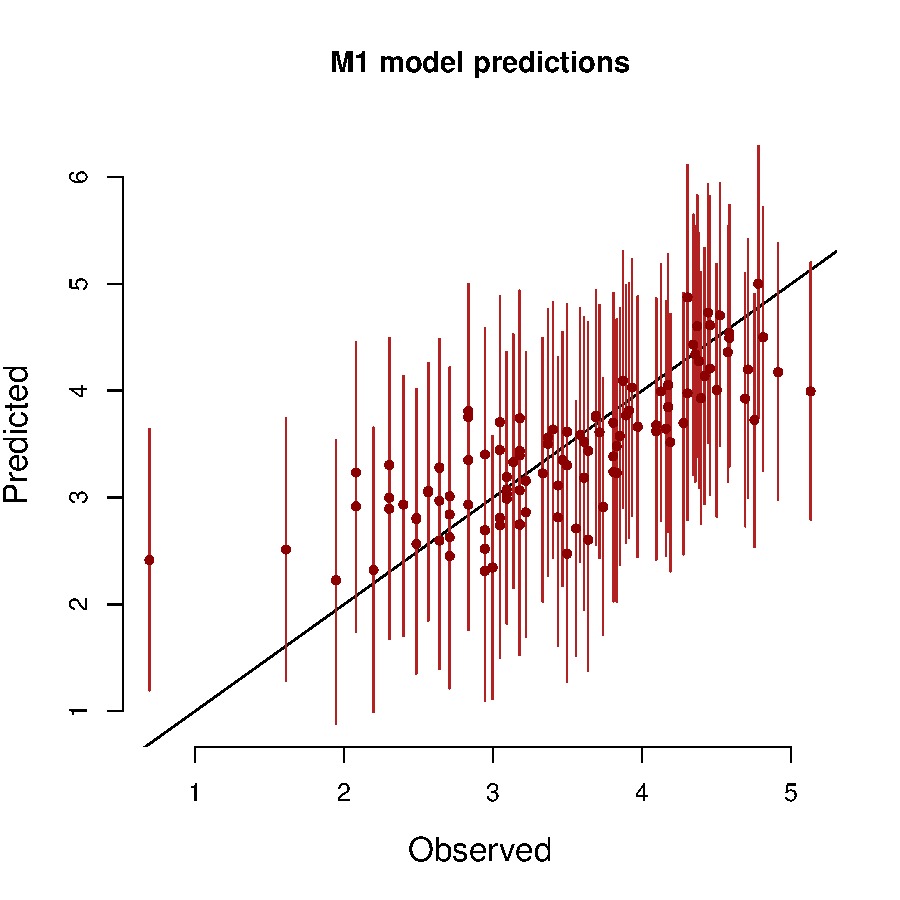
\includegraphics[scale=0.53]{figs/pred_obsfit_1.pdf}
\caption{Plot for observed versus fitted for M1. The dots are mean predictions and the lines are equal-tailed 95\% predictive intervals. The black line is the line $y=x$.}
\label{obsfit1}
\end{figure}

\begin{figure}
\centering
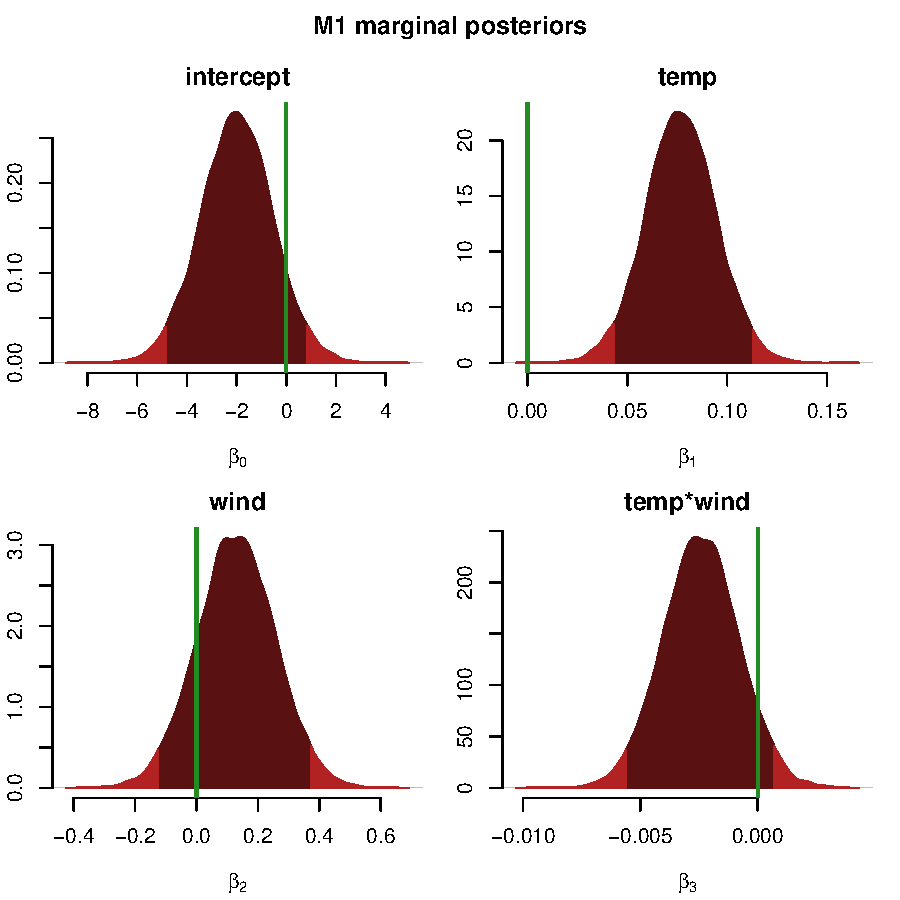
\includegraphics[scale=0.40]{figs/post_1.pdf}
\caption{Marginal posterior distributions for $\m{\beta}$ for M1. The shaded regions are the 95\% HPD intervals and the green vertical lines mark $x=0$.}
\label{post1}
\end{figure}

\begin{figure}
\centering
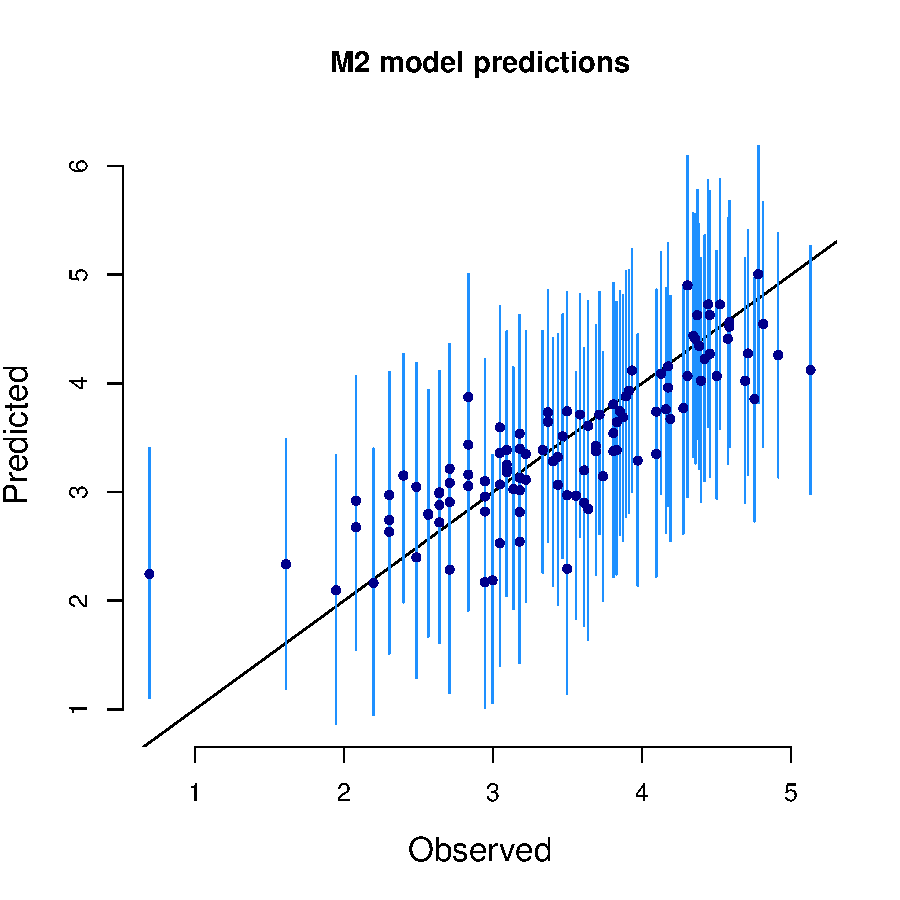
\includegraphics[scale=0.53]{figs/pred_obsfit_2.pdf}
\caption{Plot for observed versus fitted for M2. The dots are mean predictions and the lines are equal-tailed 95\% predictive intervals. The black line is the line $y=x$.}
\label{obsfit2}
\end{figure}

\begin{figure}
\centering
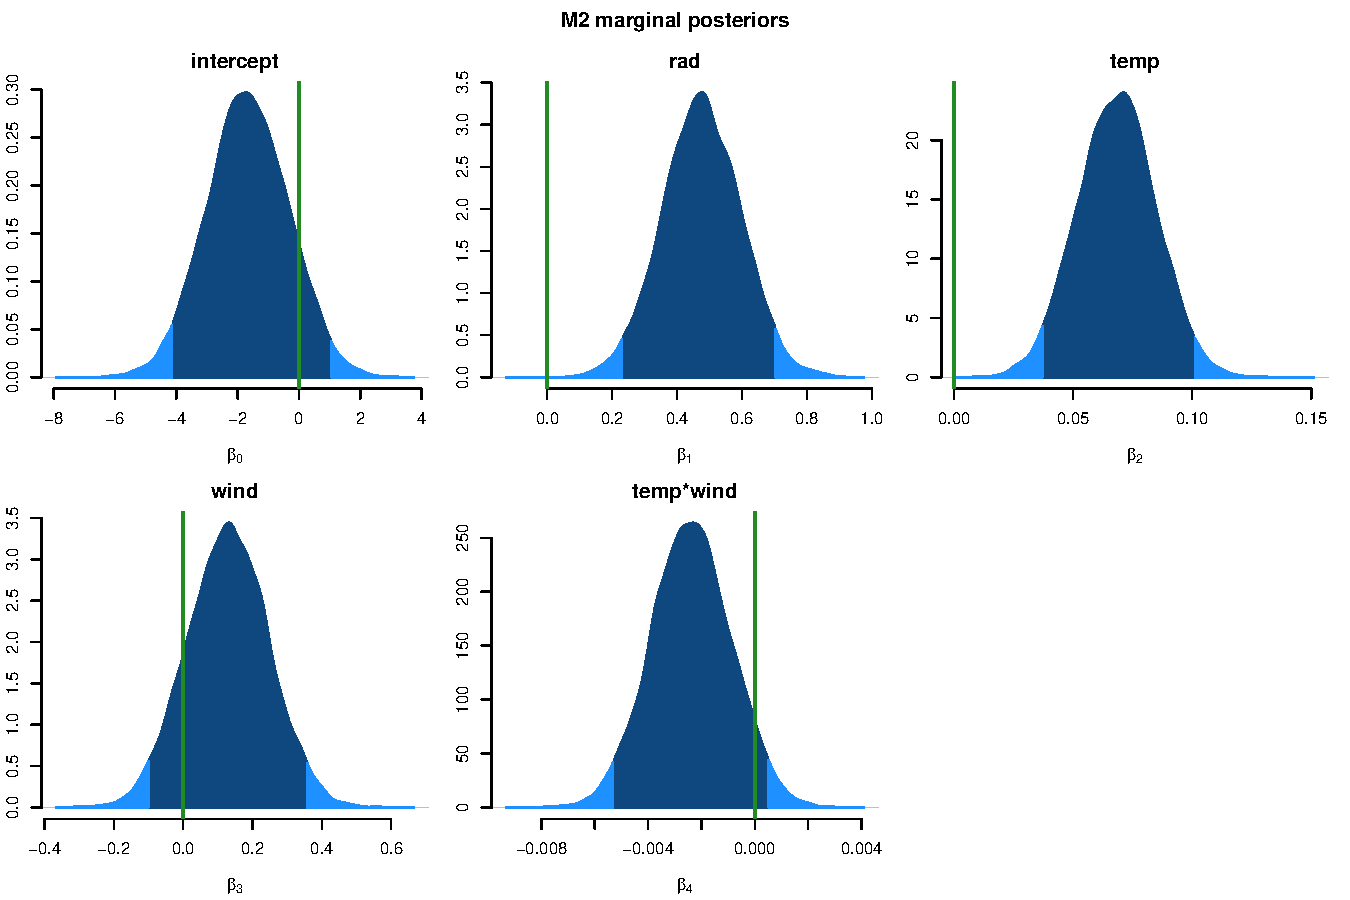
\includegraphics[scale=0.40]{figs/post_2.pdf}
\caption{Marginal posterior distributions for $\m{\beta}$ for M2. The shaded regions are the 95\% HPD intervals and the green vertical lines mark $x=0$.}
\label{post2}
\end{figure}

Table \ref{dic} provides the DIC, PPL, and K-S statistics for M1 and M2. Though DIC and PPL are considerably smaller for M2, the evidence we have considered suggests that M1 may be a better fit the data than M2. In terms of model adequacy, the only quantifiable difference we have seen is that of the $p$-values in the $\chi^2$ test and the K-S test. But both tests essentially make the same conclusion: that there is weak evidence to suggest the models do not fit. Since both provide nearly the same predictions, we prefer M2 over M1 since it has the lower DIC and we believe solar radiation makes a real contribution in explaining ozone (the marginal posterior for the radiation parameter has nearly no mass at zero).

\section{Discussion}

We have considered two models that explain ozone. The first (M1) is a function only of temperature and wind speed, while the second (M2) is a function of solar radiation, temperature, and wind speed. Both models performed very similarly in terms of predictive accuracy and goodness-of-fit. The difference in the models is in their DIC. Having a smaller DIC and significant radiation component leads us to choose M2 over M1.

In this paper, we looked at only a handful of possible measures to assess model fit and make comparisons. We chose the ones we did in part because of their relatively simple nature. They may not be the best, but then there is no golden rule on determining the best model. Based on the measures we considered, there was not enough evidence to suggest the models do not correctly predict ozone. We have seen that the models predict ozone \emph{well enough}.

A future study may incorporate expert knowledge from the climate field. Perhaps there are some non-linear relations we would expect to see in this kind of data. Or it may be a known fact there is no interaction between temperature and wind speed in explaining ozone. Such information would greatly enhance the modeling process. Under our present circumstance, we simply do not have that knowledge without having consulted an expert.

\begin{figure}
\centering
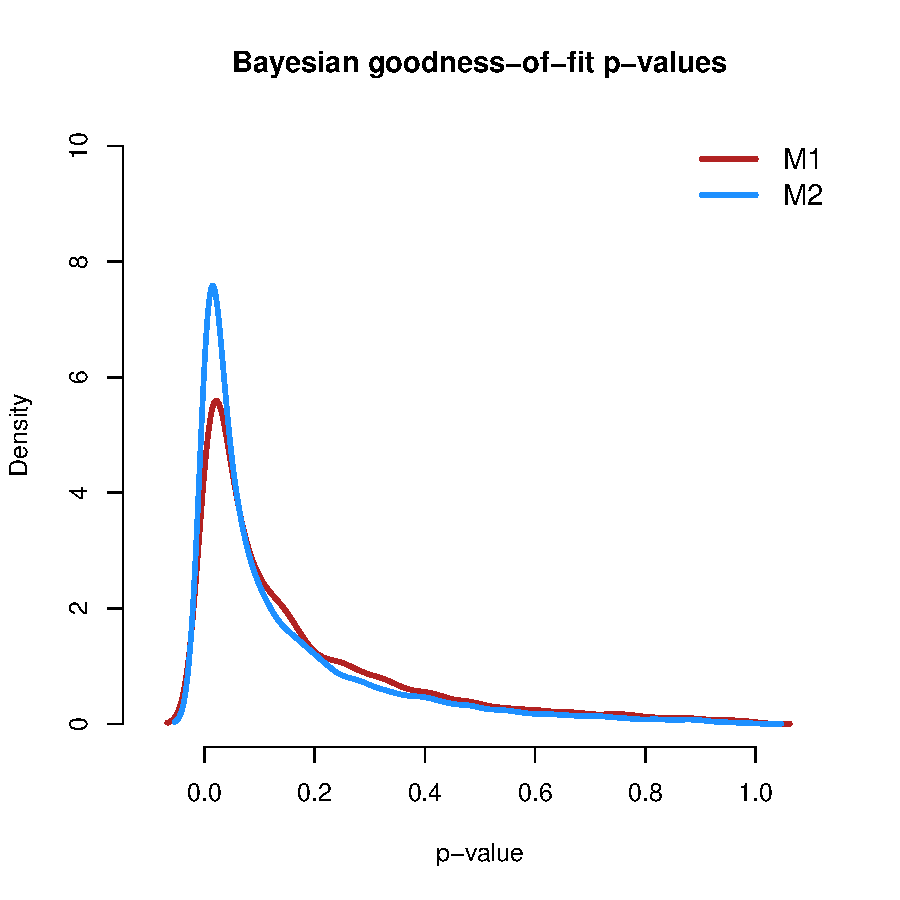
\includegraphics[scale=0.55]{figs/gof.pdf}
\caption{Distribution of $p$-values for the Bayesian goodness-of-fit test.}
\label{gof}
\end{figure}

\begin{figure}
\centering
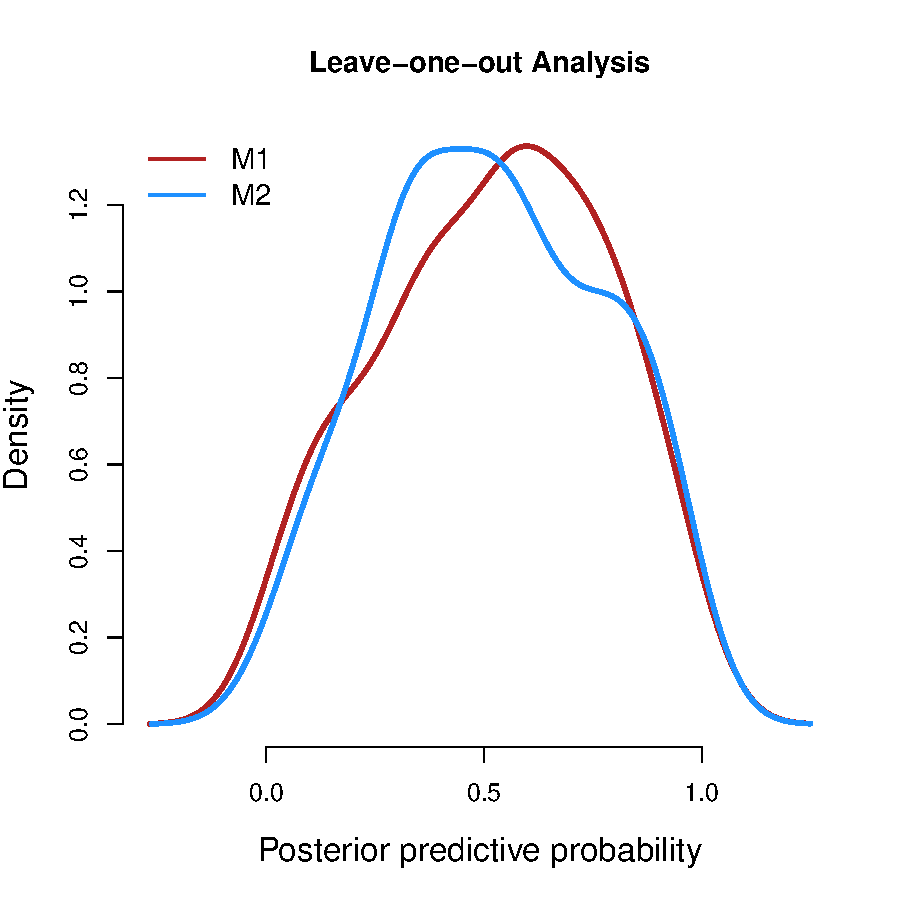
\includegraphics[scale=0.55]{figs/loo.pdf}
\caption{Distributions of the CDF evaluated at each observation based on leave-one-out cross-validation.}
\label{loo}
\end{figure}

\newpage
\onecolumn

\noindent \textbf{Code}

\begin{scriptsize}
\begin{verbatim}
source("~/files/R/mcmc/bayes_functions.R")
dat = read.table("~/files/data/fye_2016_data.txt", header = TRUE)

### Add 1 (to handle any zeroes if any) and take log transform
dat[,1] = log(dat[,1]+1)
names(dat)[1]="log(ozone+1)"

###
y = dat[,1]
rad = dat[,2]
temp = dat[,3]
wind = dat[,4]
n = length(y)

summary(dat)

#pdf("figs/pairs.pdf", width = 6, height = 6)
pairs(dat, pch = 20,
#   upper.panel = function(x, y, ...){ points(x, y, ...) },
    lower.panel = function(x, y, ...){
        cc = round(cor(x, y), 3)
        text(x = sum(range(x))/2, y = sum(range(y))/2,
            label = as.character(cc), cex=1+2.0*abs(cc))
        },
    diag.panel = function(x, ...){
        usr = par("usr"); on.exit(par(usr))
        par(usr = c(usr[1:2], 0, 1.5) )
        h = hist(x, plot = FALSE)
        breaks = h$breaks; nB <- length(breaks)
        y = h$counts; y = y/max(y)
        rect(breaks[-nB], 0, breaks[-1], y, col = "gray50", border= "white", ...)
        box()
        }
    )
#dev.off()

library(rgl)
plot3d(temp, wind, y, col = dat[,2]+1, box = FALSE, axes = FALSE,
    xlab = "", ylab = "", zlab = "", zlim = c(0, 6))
for (i in 1:11){
    lines3d(rbind(c(min(temp), min(wind)+(i-1)*diff(range(wind))/10, 0),
        c(max(temp), min(wind)+(i-1)*diff(range(wind))/10, 0)),
        col = 'gray75')
    lines3d(rbind(c(min(temp)+(i-1)*diff(range(temp))/10, min(wind), 0),
        c(min(temp)+(i-1)*diff(range(temp))/10, max(wind), 0)),
        col = 'gray75')
    }
points3d(temp, wind, y, col = dat[,2]+1, size = 5)
segments3d(rep(temp, each = 2), rep(wind, each = 2), c(rbind(0, y)),
    col = "gray30")
axis3d('x-'); mtext3d(colnames(dat)[3], 'x-', 2.5)
axis3d('y-'); mtext3d(colnames(dat)[4], 'y-', 2.5)
axis3d('z+'); mtext3d("log(ozone+1)", 'z+', 1.5, at = 3.5)
#rgl.postscript("figs/log_data.pdf", "pdf")

plot3d(temp, wind, exp(y)-1, col = dat[,2]+1, box = FALSE, axes = FALSE,
    xlab = "", ylab = "", zlab = "")
for (i in 1:11){
    lines3d(rbind(c(min(temp), min(wind)+(i-1)*diff(range(wind))/10, 0),
        c(max(temp), min(wind)+(i-1)*diff(range(wind))/10, 0)),
        col = 'gray75')
    lines3d(rbind(c(min(temp)+(i-1)*diff(range(temp))/10, min(wind), 0),
        c(min(temp)+(i-1)*diff(range(temp))/10, max(wind), 0)),
        col = 'gray75')
    }
points3d(temp, wind, exp(y)-1, col = dat[,2]+1, size = 5)
segments3d(rep(temp, each = 2), rep(wind, each = 2), c(rbind(0, exp(y)-1)),
    col = "gray30")
axis3d('x-'); mtext3d(colnames(dat)[3], 'x-', 2.5)
axis3d('y-'); mtext3d(colnames(dat)[4], 'y-', 2.5)
axis3d('z+'); mtext3d(colnames(dat)[1], 'z+', 1.5)
#rgl.postscript("figs/data.pdf", "pdf")

design.matrices = list(
    matrix(rep(1, n), n, 1, dimnames = list(NULL, "Intercept")),
    cbind("Intercept"=1, rad),
    cbind("Intercept"=1, temp),
    cbind("Intercept"=1, wind),
    cbind("Intercept"=1, rad, temp),
    cbind("Intercept"=1, rad, temp, rad*temp),
    cbind("Intercept"=1, rad, wind),
    cbind("Intercept"=1, rad, wind, rad*wind),
    cbind("Intercept"=1, temp, wind),
    cbind("Intercept"=1, temp, wind, temp*wind),
    cbind("Intercept"=1, rad, temp, wind),
    cbind("Intercept"=1, rad, temp, wind, rad*temp),
    cbind("Intercept"=1, rad, temp, wind, rad*wind),
    cbind("Intercept"=1, rad, temp, wind, temp*wind),
    cbind("Intercept"=1, rad, temp, wind, rad*temp, rad*wind),
    cbind("Intercept"=1, rad, temp, wind, rad*temp, temp*wind),
    cbind("Intercept"=1, rad, temp, wind, rad*wind, temp*wind),
    cbind("Intercept"=1, rad, temp, wind, rad*temp, rad*wind, temp*wind))
qnum = length(design.matrices)

picked.model = c(10, 14)
picked.col = c('firebrick', 'dodgerblue')

nburn = 200
nmcmc = 10000

model.DIC1 = double(qnum)
model.DIC2 = double(qnum)
model.gof = matrix(0, nmcmc, qnum)
model.ppl = matrix(0, 2, qnum)

for (model.n in 1:qnum){
    X = design.matrices[[model.n]]

    p = NCOL(X)
    prior.m = rep(0, p)
    prior.g = n
    prior.a = 0
    prior.b = 0

    A = t(X) %*% X
    max(eigen(A)$values) / min(eigen(A)$values)
    chol.A = t(chol(solve(A)))
    post.mean = 1/(prior.g + 1) * (prior.g * solve(t(X) %*% X) %*% t(X) %*% y + prior.m)

    param.beta = matrix(0, nburn + nmcmc, p)
    param.sig2 = double(nburn + nmcmc)
    param.sig2[1] = 1

    ##### Gibbs sampler
    for (i in 2:(nburn + nmcmc)){
        param.beta[i,] = post.mean +
            sqrt(prior.g * param.sig2[i-1] / (prior.g + 1)) * chol.A %*% rnorm(p, 0, 1)
        param.sig2[i] = 1/rgamma(1,
            prior.a + n/2 + p/2, 
            prior.b + 0.5*sum((y - X %*% param.beta[i,])^2) +
                0.5/prior.g * t(param.beta[i,] - prior.m) %*% A %*% (param.beta[i,] - prior.m))
        }

    # Truncate
    param.beta = tail(param.beta, nmcmc)
    param.sig2 = tail(param.sig2, nmcmc)

    ### Posterior predictions
    pred.y = matrix(0, n, nmcmc)
    for (i in 1:nmcmc)
        pred.y[,i] = rnorm(n, X %*% param.beta[i,], 1*sqrt(param.sig2[i]))

    ### DIC
    dtheta = matrix(0, nmcmc)
    for (i in 1:nmcmc)
        dtheta[i] = -2*sum(dnorm(y, X %*% param.beta[i,], sqrt(param.sig2[i]), log = TRUE))
    model.DIC1[model.n] = mean(dtheta) + var(dtheta)/2
    model.DIC2[model.n] = 2*mean(dtheta) + 2*sum(dnorm(y,
        X %*% apply(param.beta, 2, mean), sqrt(mean(param.sig2))))

    ### Bayes GOF
    model.gof[,model.n] = bayes.gof(y, cbind(param.beta, param.sig2),
        function(y, param) pnorm(y, X %*% param[1:NCOL(X)], sqrt(param[NCOL(X)+1])),
        every = nmcmc + 1)

    ### PPL
    model.ppl[1, model.n] = sum((y - apply(pred.y, 1, mean))^2)
    model.ppl[2, model.n] = sum(apply(pred.y, 1, var))

    cat("Complete:", model.n, "/", qnum, "\r")
    }
cat("\n")

### Indexes for M1 and M2 (with colors)
picked = c(10, 14)
cols.A = c('firebrick', 'dodgerblue')
cols.B = c('darkred', 'darkblue')

### Matrix for DIC and PPL
cbind(model.DIC1, t(model.ppl), apply(model.ppl, 2, sum))[picked,]

### Plot of GOF p-values
pdf("figs/gof.pdf", width = 6, height = 6)
plot(0, type='n', xlim = c(-0.1, 1.1), ylim = c(0, 10), axes = FALSE, ylab = "Density",
    main = "Bayesian goodness-of-fit p-values", xlab = "p-value")
for (j in 1:2)
    lines(density(model.gof[,picked[j]]), col = cols.A[j], lwd = 3)
legend("topright", legend = c("M1", "M2"), col = cols.A,
    box.lty = 0, lwd = 3, cex = 1.2)
axis(1)
axis(2)
apply(model.gof[,picked], 2, function(x) mean(x > 0.05))
dev.off()
\end{verbatim}
\end{scriptsize}

\bigskip
\bigskip

\noindent \textbf{Code: Leave-one-out CV}

\begin{scriptsize}
\begin{verbatim}
source("~/files/R/mcmc/bayes_functions.R")
dat = read.table("~/files/data/fye_2016_data.txt", header = TRUE)

###
z = log(dat[,1]+1)
rad = dat[,2]
temp = dat[,3]
wind = dat[,4]
m = length(z)
design.matrices = list(
#   matrix(rep(1, n), n, 1, dimnames = list(NULL, "Intercept")),
#   cbind("Intercept"=1, rad),
#   cbind("Intercept"=1, temp),
#   cbind("Intercept"=1, wind),
#   cbind("Intercept"=1, rad, temp),
#   cbind("Intercept"=1, rad, temp, rad*temp),
#   cbind("Intercept"=1, rad, wind),
#   cbind("Intercept"=1, rad, wind, rad*wind),
#   cbind("Intercept"=1, temp, wind),
    cbind("Intercept"=1, temp, wind, temp*wind),
#   cbind("Intercept"=1, rad, temp, wind),
#   cbind("Intercept"=1, rad, temp, wind, rad*temp),
#   cbind("Intercept"=1, rad, temp, wind, rad*wind),
    cbind("Intercept"=1, rad, temp, wind, temp*wind))#,
#   cbind("Intercept"=1, rad, temp, wind, rad*temp, rad*wind),
#   cbind("Intercept"=1, rad, temp, wind, rad*temp, temp*wind),
#   cbind("Intercept"=1, rad, temp, wind, rad*wind, temp*wind),
#   cbind("Intercept"=1, rad, temp, wind, rad*temp, rad*wind, temp*wind))
qnum = length(design.matrices)

funpar = function(k){
    emp.cdf = double(qnum)
    for (model.n in 1:qnum){
        y = z[-k]
        n = length(y)
        X = matrix(design.matrices[[model.n]][-k,], nrow = n)
        xstar = design.matrices[[model.n]][k,]

        nburn = 200
        nmcmc = 10000

        p = NCOL(X)
        prior.m = rep(0, p)
        prior.g = n
        prior.a = 0
        prior.b = 0

        A = t(X) %*% X
        max(eigen(A)$values) / min(eigen(A)$values)
        chol.A = t(chol(solve(A)))
        post.mean = 1/(prior.g + 1) * (prior.g * solve(t(X) %*% X) %*% t(X) %*% y + prior.m)

        param.beta = matrix(0, nburn + nmcmc, p)
        param.sig2 = double(nburn + nmcmc)
        param.sig2[1] = 1

        ##### Gibbs sampler
        for (i in 2:(nburn + nmcmc)){
            param.beta[i,] = post.mean +
                sqrt(prior.g * param.sig2[i-1] / (prior.g + 1)) * chol.A %*% rnorm(p, 0, 1)
            param.sig2[i] = 1/rgamma(1,
                prior.a + n/2 + p/2, 
                prior.b + 0.5*sum((y - X %*% param.beta[i,])^2) +
                    0.5/prior.g * t(param.beta[i,] - prior.m) %*% A %*% (param.beta[i,] - prior.m))
            }

        # Truncate
        param.beta = tail(param.beta, nmcmc)
        param.sig2 = tail(param.sig2, nmcmc)

        ### Posterior predictions
        pred.y.0 = rnorm(nmcmc, param.beta %*% xstar, sqrt(param.sig2))

        emp.cdf[model.n] = mean(pred.y.0 <= z[k])
        }
    return (emp.cdf)
    }

library(foreach)
library(doMC)
registerDoMC(4)

probs = foreach(k = 1:length(z), .combine=rbind) %dopar% funpar(k)

xlim = c(Inf, -Inf)
ylim = c(Inf, -Inf)
for (j in 1:qnum){
    dens = density(probs[,j])
    xlim[1] = min(xlim[1], dens$x)
    xlim[2] = max(xlim[2], dens$x)
    ylim[1] = min(ylim[1], dens$y)
    ylim[2] = max(ylim[2], dens$y)
    }

#pdf("figs/loo.pdf", width = 6, height = 6)
plot(0,type='n',col='firebrick',lwd=2,xlab="Posterior predictive probability",
    main="Leave-one-out Analysis",cex.lab=1.3,xlim=xlim,ylim=ylim,ylab="Density",
    axes = FALSE)
axis(1); axis(2)
lines(density(probs[,1]), col = 'firebrick', lwd = 3)
lines(density(probs[,2]), col = 'dodgerblue', lwd = 3)
legend("topleft", box.lty = 0, col = c('firebrick', 'dodgerblue'),
    legend = paste0("M", 1:qnum), lty=1, lwd = 2, cex = 1.2)
#dev.off()

### K-S test
t(t(apply(probs, 2, function(x) ks.test(jitter(x), 'punif')$p.value)))
\end{verbatim}
\end{scriptsize}



\end{document}
